


\tikzset{every picture/.style={line width=0.75pt}} %set default line width to 0.75pt        

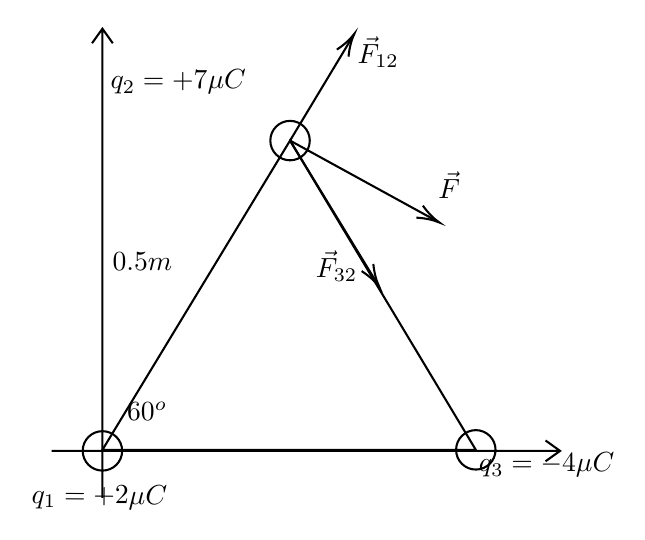
\begin{tikzpicture}[x=0.75pt,y=0.75pt,yscale=-1,xscale=1]
%uncomment if require: \path (0,300); %set diagram left start at 0, and has height of 300

%Shape: Triangle [id:dp9976522048032088] 
\draw   (267,67.5) -- (356.5,216.5) -- (176.6,216.5) -- cycle ;
%Shape: Circle [id:dp5539049513903027] 
\draw   (167.1,217) .. controls (167.1,211.75) and (171.35,207.5) .. (176.6,207.5) .. controls (181.85,207.5) and (186.1,211.75) .. (186.1,217) .. controls (186.1,222.25) and (181.85,226.5) .. (176.6,226.5) .. controls (171.35,226.5) and (167.1,222.25) .. (167.1,217) -- cycle ;
%Shape: Circle [id:dp03557687797226117] 
\draw   (347,216.5) .. controls (347,211.25) and (351.25,207) .. (356.5,207) .. controls (361.75,207) and (366,211.25) .. (366,216.5) .. controls (366,221.75) and (361.75,226) .. (356.5,226) .. controls (351.25,226) and (347,221.75) .. (347,216.5) -- cycle ;
%Shape: Axis 2D [id:dp35701988623397174] 
\draw  (152.1,217) -- (397.1,217)(176.6,13.6) -- (176.6,239.6) (390.1,212) -- (397.1,217) -- (390.1,222) (171.6,20.6) -- (176.6,13.6) -- (181.6,20.6)  ;
%Shape: Circle [id:dp21574096627013728] 
\draw   (257.5,67.5) .. controls (257.5,62.25) and (261.75,58) .. (267,58) .. controls (272.25,58) and (276.5,62.25) .. (276.5,67.5) .. controls (276.5,72.75) and (272.25,77) .. (267,77) .. controls (261.75,77) and (257.5,72.75) .. (257.5,67.5) -- cycle ;
%Straight Lines [id:da743332007005598] 
\draw    (267,67.5) -- (308.96,136.29) ;
\draw [shift={(310,138)}, rotate = 238.62] [color={rgb, 255:red, 0; green, 0; blue, 0 }  ][line width=0.75]    (10.93,-3.29) .. controls (6.95,-1.4) and (3.31,-0.3) .. (0,0) .. controls (3.31,0.3) and (6.95,1.4) .. (10.93,3.29)   ;
%Straight Lines [id:da4895454589919841] 
\draw    (267,67.5) -- (337.25,106.04) ;
\draw [shift={(339,107)}, rotate = 208.75] [color={rgb, 255:red, 0; green, 0; blue, 0 }  ][line width=0.75]    (10.93,-3.29) .. controls (6.95,-1.4) and (3.31,-0.3) .. (0,0) .. controls (3.31,0.3) and (6.95,1.4) .. (10.93,3.29)   ;

%Straight Lines [id:da8197536808983341] 
\draw    (267,67.5) -- (296.97,17.71) ;
\draw [shift={(298,16)}, rotate = 121.05] [color={rgb, 255:red, 0; green, 0; blue, 0 }  ][line width=0.75]    (10.93,-3.29) .. controls (6.95,-1.4) and (3.31,-0.3) .. (0,0) .. controls (3.31,0.3) and (6.95,1.4) .. (10.93,3.29)   ;

% Text Node
\draw (179,32) node [anchor=north west][inner sep=0.75pt]    {$q_{2} =+7\mu C$};
% Text Node
\draw (298,16) node [anchor=north west][inner sep=0.75pt]    {$\vec{F}_{12}$};
% Text Node
\draw (337,81) node [anchor=north west][inner sep=0.75pt]    {$\vec{F}$};
% Text Node
\draw (278,119) node [anchor=north west][inner sep=0.75pt]    {$\vec{F}_{32}$};
% Text Node
\draw (187,192) node [anchor=north west][inner sep=0.75pt]    {$60^{o}$};
% Text Node
\draw (180,120) node [anchor=north west][inner sep=0.75pt]    {$0.5m$};
% Text Node
\draw (356.5,216.5) node [anchor=north west][inner sep=0.75pt]    {$q_{3} =-4\mu C$};
% Text Node
\draw (141.09,231.66) node [anchor=north west][inner sep=0.75pt]  [rotate=-0.42]  {$q_{1} =+2\mu C$};


\end{tikzpicture}
